\documentclass[10pt,letterpaper]{article}
\renewcommand{\rmdefault}{ptm}

\usepackage[left=1in,right=1in,top=1in,bottom=1in]{geometry} 
\usepackage{amsmath}
\usepackage{amsfonts}
\usepackage{amsthm}
\usepackage{amssymb}
\usepackage{polynomial}
\usepackage{layouts}
\usepackage{enumerate}
\usepackage{syntax}
\usepackage{gensymb}
\usepackage{enumitem}
\usepackage{cancel}
\usepackage{calc}
\usepackage{enumerate}
\usepackage{xcolor}

\usepackage{minted}

\usepackage[version=0.96]{pgf}
\usepackage{tikz}
\usetikzlibrary{arrows,shapes,automata,backgrounds,petri,positioning}
\usetikzlibrary{decorations.pathmorphing}
\usetikzlibrary{decorations.shapes}
\usetikzlibrary{decorations.text}
\usetikzlibrary{decorations.fractals}
\usetikzlibrary{decorations.footprints}
\usetikzlibrary{shadows}
\usetikzlibrary{calc}
\usetikzlibrary{spy}
\usetikzlibrary{matrix}

\usepackage{tikz-qtree}

\setcounter{tocdepth}{2}
\setcounter{secnumdepth}{4}
\usepackage[bookmarksopen,bookmarksdepth=3]{hyperref}
\usepackage{titlesec}


%define new colors
\definecolor{dark-red}{rgb}{0.8,0.15,0.15}
\definecolor{dark-blue}{rgb}{0.15,0.15,0.7}
\definecolor{medium-blue}{rgb}{0,0,0.5}
\definecolor{dark-green}{rgb}{0.2,0.7,0.7}

%set up color for table of contents
\hypersetup{
    colorlinks, linkcolor={dark-green},
    citecolor={dark-blue}, urlcolor={medium-blue}
}

\usepackage{tocloft}

%preven linebreak between subsection header and its content
\titleformat{\subsection}[runin]{\normalfont\bfseries}{\thesubsection.}{2pt}{}
%\titleformat{\section}[runin]{\normalfont\bfseries\filcenter}{\thesection.}{5pt}{}


\titleformat{\section}[block]
{\normalfont\sffamily\LARGE}
{\thesection}{.2em}{\titlerule\\[.2ex]\bfseries}

%title
\title{\textbf{Math 350 - Advanced Calculus \\ Homework 4}}
\author{Chan Nguyen}

%set numwidth of section
\setlength{\cftsecnumwidth}{1.5cm} 
%make subsection numwidth different than as section
\setlength{\cftsubsecnumwidth}{3cm}
%make subsection indent the same as section
\setlength{\cftsubsecindent}{\cftsecindent} 

\newcommand{\sol}{\textbf{Solution}}

\usepackage{tikz}
\usetikzlibrary{matrix}
\usetikzlibrary{shapes,backgrounds}

\makeatletter
\newcommand{\DESCRIPTION@original@item}{}
\let\DESCRIPTION@original@item\item
\newcommand*{\DESCRIPTION@envir}{DESCRIPTION}
\newlength{\DESCRIPTION@totalleftmargin}
\newlength{\DESCRIPTION@linewidth}
\newcommand{\DESCRIPTION@makelabel}[1]{\llap{#1}}%
\newcommand{\DESCRIPTION@item}[1][]{%
  \setlength{\@totalleftmargin}%
       {\DESCRIPTION@totalleftmargin+\widthof{\textbf{#1 }}-\leftmargin}%
  \setlength{\linewidth}
       {\DESCRIPTION@linewidth-\widthof{\textbf{#1 }}+\leftmargin}%
  \par\parshape \@ne \@totalleftmargin \linewidth
  \DESCRIPTION@original@item[\textbf{#1}]%
}
\newenvironment{DESCRIPTION}
  {\list{}{\setlength{\labelwidth}{0cm}%
           \let\makelabel\DESCRIPTION@makelabel}%
   \setlength{\DESCRIPTION@totalleftmargin}{\@totalleftmargin}%
   \setlength{\DESCRIPTION@linewidth}{\linewidth}%
   \renewcommand{\item}{\ifx\@currenvir\DESCRIPTION@envir
                           \expandafter\DESCRIPTION@item
                        \else
                           \expandafter\DESCRIPTION@original@item
                        \fi}}
  {\endlist}
\makeatother

\begin{document}

\tableofcontents 
\maketitle

\setlength{\parindent}{0pt}
\setlength{\parskip}{1ex}
	\phantomsection
	\subsection*{{\color{red}\underline{Problem 1}}}
	\addcontentsline{toc}{subsection}{\numberline{}Problem 1}
	\begin{enumerate}[label=(\roman{*})]
		\item Prove that if $a_n < b_n$ and $\displaystyle\lim_{n\to \infty}a_n = a$ and $\displaystyle\lim_{n\to\infty}b_n = b$
		then $a \leq b$
		\item Prove that if $a_n \leq c_n \leq b_n$ and $\displaystyle\lim_{n\to \infty}a_n = \displaystyle\lim_{n\to \infty}b_n = L$, then
		$\displaystyle\lim_{n\to \infty}c_n = L$
	\end{enumerate}
	\sol
	\begin{enumerate}[label=(\roman{*})]
		\item First, we introduce two claims:
		\begin{itemize}
			\item Claim 1: If $\displaystyle\lim_{n\to\infty} a_n = a$ and 
			$\displaystyle\lim_{n\to\infty} b_n = b$ then
			$\displaystyle\lim_{n\to\infty} (a_n - b_n) = a - b$
			\item Claim 2: If the limit of $(a_n)$ exists and $a_n \geq 0$ then $\displaystyle\lim_{n\to\infty} a_n \geq 0$.
		\end{itemize}
		Claim 1:
		\begin{proof}
			By definition of limit, for $\epsilon > 0$, there exist $N_1, N_2$ such that for all $n > N_1$ and $n > N_2$
			$$|a_n - a| \leq \dfrac{\epsilon}{2} \,\,\, \text{ and } 
			\, \, \, |b_n - b| \leq \dfrac{\epsilon}{2}$$
			Let $N = \mathrm{max}(N_1, N_2)$ then for all $n \geq N$, we have
			$$|(a_n - b_n) - (a - b)| = |(a_n - a) - (b_n - b)| \leq 
			|a_n - a| + |b_n - b| < \dfrac{\epsilon}{2} + \dfrac{\epsilon}{2} = \epsilon$$ 
			
		\end{proof}
		Claim 2:
		\begin{proof}
			Let $\displaystyle\lim_{n\to\infty} a_n = M$. Suppose that $a_n \geq 0$ but $M < 0$. Let
			$$\epsilon = -\dfrac{M}{2}$$
			since $M < 0 \rightarrow -\dfrac{M}{2} > 0 \rightarrow \epsilon > 0$.
			By definition of limit,
			$$|a_n - M| < -\dfrac{M}{2}$$
			which implies $a_n - M < -\dfrac{M}{2} \Leftrightarrow a_n < -\dfrac{M}{2} + M 
			\Leftrightarrow a_n < \dfrac{M}{2}$.
			In other words, $a_n < 0$ which is a contradiction. Therefore,
			$$\displaystyle\lim_{n\to\infty} a_n \geq 0$$ 		 
		\end{proof}
		Now we are ready for the original problem! Consider the sequence $(c_n)$ where
		$$c_n = b_n - a_n$$
		since $b_n > a_n$, we must have $c_n > 0$, then from \textbf{Claim 1} and \textbf{Claim 2} we have
		$$\displaystyle\lim_{n\to\infty} c_n = \displaystyle\lim_{n\to\infty}b_n - \displaystyle\lim_{n\to\infty}a_n = 
		b - a > 0$$
		which implies $b > a$.
		\item Prove that if $a_n \leq c_n \leq b_n$ and $\displaystyle\lim_{n\to \infty}a_n = \displaystyle\lim_{n\to \infty}b_n = L$, then $\displaystyle\lim_{n\to \infty}c_n = L$
		\begin{proof}
			By definition of limit, for all $\epsilon > 0$ there exists $N_1 \in \mathbf{N}$ for all $n \geq N_1$, 
			then $|a_n - L| < \epsilon$ and there exists $N_2 \in mathbf{N}$ for all $n \geq N_2$ then 
			$|b_n - L| < \epsilon$. Let $N = \max(N_1, N_2)$, then for all $n > N$, we have
			$$|a_n - L| < \epsilon \text{ and } |b_n - L| < \epsilon$$
			Consider 
			\begin{eqnarray*}
				&&		a_n \leq c_n \leq b_n \\
	& \Leftrightarrow & a_n - L \leq c_n - L \leq b_n - L \\
	& \Leftrightarrow & -\epsilon < a_n - L \leq c_n - L \leq b_n - L < \epsilon \\
	& \Leftrightarrow & -\epsilon < c_n - L < \epsilon \\    
			\end{eqnarray*}
			$$\therefore \displaystyle\lim_{n\to\infty} c_n = L$$
		\end{proof}
	\end{enumerate}
	
	\phantomsection
	\subsection*{{\color{red}\underline{Problem 2}}}
	\addcontentsline{toc}{subsection}{\numberline{}Problem 2}
	Prove that
	\begin{enumerate}[label=(\roman{*})]
		\item $\displaystyle\lim_{n\to \infty}\dfrac{3n^3 + 7n^2 + 1}{4n^3 - 8n + 63} = \dfrac{3}{4}$
		\item $\displaystyle\lim_{n\to \infty} \dfrac{2^n + (-1)^n}{2^{n+1} + (-1)^{n+1}} = \dfrac{1}{2}$
	\end{enumerate}
	\sol
	\begin{enumerate}[label=(\roman{*})]
		\item $\displaystyle\lim_{n\to \infty}\dfrac{3n^3 + 7n^2 + 1}{4n^3 - 8n + 63} = \dfrac{3}{4}$
		\begin{proof}
			Divide both numerator and denominator by $n^3$
			\begin{eqnarray*}
				\displaystyle\lim_{n\to \infty}\dfrac{3n^3 + 7n^2 + 1}{4n^3 - 8n + 63} &=&
				\displaystyle\lim_{n\to \infty}\dfrac{3 + \dfrac{7}{n} + \dfrac{1}{n^3}}
				{4 - \dfrac{8}{n^2} + \dfrac{63}{n^3}}= \dfrac{3}{4}
			\end{eqnarray*}
		\end{proof}
		\item $\displaystyle\lim_{n\to \infty} \dfrac{2^n + (-1)^n}{2^{n+1} + (-1)^{n+1}} = \dfrac{1}{2}$
		\begin{proof}
			We have,
			\begin{eqnarray*}
				\displaystyle\lim_{n\to \infty} \dfrac{2^n + (-1)^n}{2^{n+1} + (-1)^{n+1}} &=&
				\displaystyle\lim_{n\to \infty} \dfrac{2^n}{2^{n+1} + (-1)^{n+1}} + 
				\displaystyle\lim_{n\to \infty} \dfrac{(-1)^n}{2^{n+1} + (-1)^{n+1}} \\
				&=&\displaystyle\lim_{n\to \infty} \dfrac{2^n}{2^{n+1} + (-1)^{n+1}} + 0 \\
				&=&\displaystyle\lim_{n\to \infty} \dfrac{2^n}{2^{n+1} + (-1)^{n+1}} \\
			\end{eqnarray*}
			There are two cases that we need to consider: $(-1)^n$ is either -1 or 1,
			\begin{itemize}
			\item If $n$ is even, then $(-1)^{n+1} = -1$, 
			\begin{eqnarray*}
				\displaystyle\lim_{n\to \infty} \dfrac{2^n}{2^{n+1} + (-1)^{n+1}}  &=&
				\displaystyle\lim_{n\to \infty} \dfrac{2^n}{2^{n+1} - 1} 
				\geq  \displaystyle\lim_{n\to \infty} \dfrac{2^n}{2^{n+1}} = \dfrac{1}{2}\\
			\end{eqnarray*}
			
			\item If $n$ is odd, then $(-1)^{n+1} = 1$, 
			\begin{eqnarray*}
				\displaystyle\lim_{n\to \infty} \dfrac{2^n}{2^{n+1} + (-1)^{n+1}}  &=&
				\displaystyle\lim_{n\to \infty} \dfrac{2^n}{2^{n+1} + 1} 
				\leq  \displaystyle\lim_{n\to \infty} \dfrac{2^n}{2^{n+1}} = \dfrac{1}{2}\\
			\end{eqnarray*}
			\end{itemize}
			Combine these two cases, we have
			$\dfrac{1}{2} \leq \displaystyle\lim_{n\to \infty} \dfrac{2^n}{2^{n+1} + (-1)^{n+1}} \leq \dfrac{1}{2}$.
			By Squeeze's Theorem (Sandwich's Lemma), 
			$\displaystyle\lim_{n\to \infty} \dfrac{2^n}{2^{n+1} + (-1)^{n+1}} = \dfrac{1}{2}$
		\end{proof}
	\end{enumerate}
	
	\phantomsection
	\subsection*{{\color{red}\underline{Problem 3}}}
	\addcontentsline{toc}{subsection}{\numberline{}Problem 3}
	Prove that if $a > 0$, then $\displaystyle\lim_{n\to \infty} \sqrt[n]{a} = 1$ \\
	\sol 
	\begin{proof}
	If $a = 1$, there is nothing to prove! \\
	If $0 < a < 1$, the we can consider $a = \dfrac{1}{b}$ for some $b \neq 0$ then the limit becomes
	$\displaystyle\lim_{n\to\infty}\sqrt[n]{\dfrac{1}{b}} = 
	\displaystyle\lim_{n\to\infty} \dfrac{1}{\sqrt[n]{\dfrac{1}{b}}}$
	which deduce to case $a > 1$ because if $0 < a < 1$ then $\dfrac{1}{a} > 1$.
	If $a > 1$ then $\sqrt[n]{a} > 1$. Let $\sqrt[n]{a} = (1 + x)$ for some $x > 0$. Hence
	$$(\sqrt[n]{a})^n = (1 + x)^n \Leftrightarrow a = (1 + x)^n$$
	Look at the binomial expansion of $(1 + x)^n$,
	$$(1 + x)^n = 1 + nx + \underbrace{\dbinom{n}{2}x^2 + \dbinom{n}{3}x^3 + \ldots \dbinom{n}{n}x^n
	}_{\geq 0}$$
	which tells us that $(1 + x)^n \geq 1 + nx$ for $x \geq 0$. Thus
	$$(1 + x)^n = a > 1 + nx \Rightarrow \dfrac{a - 1}{n} > x$$
	Adding $1 < \sqrt[n]{a}$ to obtain:
	$$1 < \sqrt[n]{a} = 1 + x < 1 + \dfrac{a - 1}{n}$$
	It's easy to see that 
	$$\displaystyle\lim_{n\to\infty} \bigg(1 + \dfrac{a - 1}{n}\bigg) = 1$$
	Applying "Sandwich" lemma, we have:
	$$\displaystyle\lim_{n\to\infty} \sqrt[n]{a} = 1$$
	\end{proof}
	
	\phantomsection
	\subsection*{{\color{red}\underline{Problem 4}}}
	\addcontentsline{toc}{subsection}{\numberline{}Problem 4}
	Prove that $\displaystyle\lim_{n\to \infty} \sqrt[n]{n} = 1$. (Hint: put $\sqrt[n]{n} = 1 + a_n$, prove that
	$a_n > 0$ for $n > 1$, deduce that $n - 1 \geq \dfrac{1}{2}n(n - 1)a_n^2$ for $n > 1$ hence $0 \leq a_n^2 \leq \dfrac{2}{n}$)\\
	\sol
	\begin{proof}
	Let $\sqrt[n]{n} = 1 + a_n \Rightarrow (\sqrt[n]{n})^n = (1 + a_n)^n \Rightarrow n = (1 + a_n)^n$. Using Binomial theorem,
	we have that:
	$$n \geq \dfrac{n(n - 1)}{2}a_n^2 \text{ for } n > 1$$
	Hence,
	$$a_n^2 \leq \dfrac{2}{n - 1}$$ 
	where $a_n^2 \geq 0$, so $0 \leq a_n^2 \leq \dfrac{2}{n - 1} \Rightarrow 0 \leq a_n \leq \sqrt{\dfrac{2}{n-1}}$\\ 
	Next we consider the limit,
	$$\displaystyle\lim_{n\to \infty}  \sqrt{\dfrac{2}{n-1}} = 0$$
	Apply Squeeze's Theorem (Sandwich Lemma) for $a_n$, $$0 \leq a_n \leq 0$$, then we must have
	$$\displaystyle\lim_{n\to \infty}  a_n = 0$$
	where $\sqrt[n]{n} = a_n + 1$ which implies $\displaystyle\lim_{n\to \infty} \sqrt[n]{n} = 1$
	\end{proof}
	
	\phantomsection
	\subsection*{{\color{red}\underline{Problem 5}}}
	\addcontentsline{toc}{subsection}{\numberline{}Problem 5}
	Does the sequences $a_1, a_2, a_3 \ldots$ converge or diverge? If it converges, what is the limit?
	\begin{enumerate}[label=(\roman{*})]
		\item $a_n = \dfrac{n}{n + 1} - \dfrac{n + 1}{n}$
		\item $a_n = \dfrac{2^n}{n!}$
		\item $a_n$ the $n$th decimal digit of $\sqrt{2}$ (thus $a_1 = 4, a_2 = 1, a_3 = 4, a_4 = 2 \ldots$ and so on).
	\end{enumerate}
	\sol
	\begin{enumerate}[label=(\roman{*})]
		\item $a_n = \dfrac{n}{n + 1} - \dfrac{n + 1}{n}$ converges. 
		\begin{proof}
			\begin{eqnarray*}
				\displaystyle\lim_{n\to \infty} a_n &=&
				\displaystyle\lim_{n\to \infty} \bigg(\dfrac{n}{n + 1} - \dfrac{n + 1}{n}\bigg) \\
				&=& \displaystyle\lim_{n\to \infty} \dfrac{n^2 - (n + 1)^2}{n(n + 1)} \\
				&=& \displaystyle\lim_{n\to \infty} \dfrac{(n - n - 1)(n + n + 1)}{n(n + 1)} \\
				&=& \displaystyle\lim_{n\to \infty} \dfrac{-(\dfrac{2}{n} + \dfrac{1}{n^2})}{1 + \dfrac{1}{n}}
				= \dfrac{0}{1} = 0 \\
			\end{eqnarray*}
		\end{proof}
		\item $a_n = \dfrac{2^n}{n!}$ converges.
		\begin{proof}
			Consider $$\dfrac{2 \cdot 2 \cdot 2 \cdots 2}{1 \cdot 2 \cdot 3 \cdots n} \leq 
			\dfrac{2}{1} \cdot \dfrac{2}{n} \text{ since } \dfrac{2 \cdot 2 \cdots 2}{2 \cdot 3 \cdots (n - 1)} < 1$$
			In addition, we have that:
			$$\dfrac{1}{n!} \leq \dfrac{2^n}{n!}$$
			where
				$$\displaystyle\lim_{n\to \infty} \dfrac{1}{n!} = 0 = \displaystyle\lim_{n\to \infty} 2 \cdot \dfrac{2}{n}$$
			which implies
				$$0 \leq \dfrac{2^n}{n!} \leq 0$$			
			Hence, by Squeeze's Theorem (Sandwich's Lemma)
			$$\displaystyle\lim_{n\to \infty} \dfrac{2^n}{n!} = 0$$	
		\end{proof}
		
		\item $a_n$ the $n$th decimal digit of $\sqrt{2}$ (thus $a_1 = 4, a_2 = 1, a_3 = 4, a_4 = 2 \ldots$ and so on).
		\begin{proof}
			Assume that we know $\sqrt{2}$ is irrational where $a_n \in D = \{0, 1, 2, 3, 4, 5, 6, 7, 8, 9\}$, if 
			$a_n$ converge, then the number would be of the form:
			$$d.d_1d_3d_4d_id_id_i \ldots$$
			Suppose that it converges, thus the limit exits:
			$$\displaystyle\lim_{n\to\infty}a_n = d, \text{ for some } d \in D$$
			By definition of limit, for all $\epsilon > 0$, there exits a $N \in \mathbf{N}$ such that
			for all $n > N$:
				$$|a_n - d| < \epsilon$$
			Pick $\epsilon = 1 \rightarrow |a_n - d| < 1$ where $a_n, d$ are decimal digits which is in $D$.
			The only way for $|a_n - d| < 1$ is when $a_n = d$ which is clearly a contradiction because this implies
			$\sqrt{2}$ is rational. Therefore, $n$th decimal digit of $\sqrt{2}$ does not converge.
					
		\end{proof}
	\end{enumerate}
	
	\phantomsection
	\subsection*{{\color{red}\underline{Problem 6}}}
	\addcontentsline{toc}{subsection}{\numberline{}Problem 6}
	Prove or give a counterexample. Let $a_1, a_2, \ldots$ be a sequence such that 
	$\displaystyle\lim_{n\to \infty}(a_{n+1} - a_n) = 0$. Does $a_n$ have to converge? \\
	\sol \\
	This is false. A counterexample could be:
			$$a_n = \sqrt{n}$$
		The limit of $a_{n+1} - a_{n}$ is:
		\begin{eqnarray*}
			\displaystyle\lim_{n\to \infty} (\sqrt{n+1} - \sqrt{n})
			&=& \displaystyle\lim_{n\to \infty} 
			\bigg(\dfrac{(\sqrt{n+1})^2 - (\sqrt{n})^2}{\sqrt{n+1} + \sqrt{n}}\bigg) \\
			&=& \displaystyle\lim_{n\to \infty} 
			\bigg(\dfrac{n + 1 - n}{\sqrt{n+1} + \sqrt{n}}\bigg) \\
			&=& \displaystyle\lim_{n\to \infty} 
			\bigg(\dfrac{1}{\sqrt{n+1} + \sqrt{n}}\bigg) = 0
		\end{eqnarray*}
		but $$ \displaystyle\lim_{n\to \infty} \sqrt{n} = \infty$$
	
	\phantomsection
	\subsection*{{\color{red}\underline{Problem 7}}}
	\addcontentsline{toc}{subsection}{\numberline{}Problem 7}
	Prove that the sequence $x_1, x_2, x_3 \ldots$ of real numbers defined by $x_1 = 1$ and $x_{n+1} = x_n + \dfrac{1}{x_n^2}$
	is unbounded. \\
	\sol 
	\begin{proof}
		Prove by contradiction: \\
		Suppose that the limit of this sequence exists, then by definition of limit, for all $\epsilon > 0$, there exists 
		a natural number $N$ such that for all $n > N$ then $|x_n - L| < \epsilon$. But there is no such $\epsilon$ because
		$x_{n+1} > x_{n}$. We will prove this by induction: \\
		Base case, 
			$$x_{2} = 1 + \dfrac{1}{1^2} = 1 + 1 = 2$$ 
		Inductive hypothesis,
			$$x_{n} > x_{n - 1}$$
		Consider,
			$$x_{n+1} = x_n + \dfrac{1}{x_n^2}$$
		where $\dfrac{1}{x_n^2} > 0$ 
		Thus $$x_{n+1} > x_n$$
		Therefore the limit doesn't exists. \\
		Another way to prove it is to consider the following fact: "If the limit exists, it must satisfy an algebraic expression". 
		In other words, if the sequence converge we will have $x_n = x_{n - 1}$, 
		$$x_n = x_n + \dfrac{1}{x_n^2}$$ 
		Cancel $x_n$ from both sides of the equation, we obtain:
		$$0 = \dfrac{1}{x_n^2}$$
		which is impossible, thus we have a contradiction.
		
	\end{proof}
	
	\phantomsection
	\subsection*{{\color{red}\underline{Problem 8}}}
	\addcontentsline{toc}{subsection}{\numberline{}Problem 8}
	Prove or give a counterexample
	\begin{enumerate}[label=(\roman{*})]
		\item If $(a_n)$ is a non-decreasing sequence that is $a_1 \leq a_2 \leq a_3 \leq \ldots$ such that
		$\displaystyle\lim_{n\to \infty}(a_{n+1} - a_n) = 0$, then $(a_n)$ is convergent.
		\item If $(a_n)$ is non-decreasing and bounded above, and $\displaystyle\lim_{n\to \infty}a_n = a$ then $a_n \leq a$
	\end{enumerate}
	\sol
	\begin{enumerate}[label=(\roman{*})]
		\item This is false. A counterexample would be the same as problem 6.
			$$a_n = \sqrt{n}$$
		because a non-decreasing sequence is also an increasing sequence.
		However if we want to be more precise about the equal sign, we could choose
			$$a_n = \sqrt{\bigg\lfloor \dfrac{n}{2} \bigg\rfloor}$$
		Apparently, 
			$$\displaystyle\lim_{n\to\infty} a_n = \infty$$
		What we need to show is that 
			$$\displaystyle\lim_{n\to\infty} a_{n+1} - a_{n} = 0$$
		There are two cases that we need to consider:
		\begin{itemize}
			\item $n \pmod{2} \equiv 0 \rightarrow n = 2k$ for some positive integers $k$. We have,
			$$a_{n} = \sqrt{\bigg\lfloor \dfrac{2k}{2} \bigg\rfloor} = \sqrt{2k/2} = \sqrt{k}$$
			$$a_{n+1} = \sqrt{\bigg\lfloor \dfrac{2k+1}{2} \bigg\rfloor} = \sqrt{k}$$ 
			This case is trivial since 
				$$\displaystyle\lim_{n\to\infty} (a_{n+1} - a_{n}) 
				\displaystyle\lim_{n\to\infty} (\sqrt{k} - \sqrt{k}) = 0$$
			\item $n \pmod{2} \equiv 1 \rightarrow n = 2k + 1$ for some positive integers $k$. We have,
			 $$a_{n} = \sqrt{\bigg\lfloor \dfrac{2k+1}{2} \bigg\rfloor} = \sqrt{k}$$
			 $$a_{n} = \sqrt{\bigg\lfloor \dfrac{2k+1+1}{2} \bigg\rfloor} = \sqrt{k+1}$$
			 Note that as $n \rightarrow \infty$, so does $k \rightarrow infty$, so 
			 we can replace the $n$ in the limit as $k$.
			\begin{eqnarray*}
			\displaystyle\lim_{n\to \infty} (a_{n+1} - a_{n}) 
			&=& \displaystyle\lim_{k\to \infty} (\sqrt{k+1} - \sqrt{k}) \\
			&=& \displaystyle\lim_{k\to \infty} 
			\bigg(\dfrac{(\sqrt{k+1})^2 - (\sqrt{k})^2}{\sqrt{k+1} + \sqrt{k}}\bigg) \\
			&=& \displaystyle\lim_{k\to \infty} 
			\bigg(\dfrac{k + 1 - k}{\sqrt{k+1} + \sqrt{k}}\bigg) \\
			&=& \displaystyle\lim_{k\to \infty} 
			\bigg(\dfrac{1}{\sqrt{k+1} + \sqrt{k}}\bigg)\\
			&=& \dfrac{1}{\infty} = 0
			\end{eqnarray*}  
		\end{itemize}
			
		\item If $(a_n)$ is non-decreasing and bounded above, and $\displaystyle\lim_{n\to \infty}a_n = a$ then $a_n \leq a$		
		\begin{proof}
			Since $(a_n)$ is bounded above, there exists a least upper bound for $(a_n)$. Let $\sup((a_n)) = M$, we will
			show that $M$ is actually $a$. 
			By definition of the least upper bound, we know that $a_n \leq M$ for all $n \in \mathbf{N}$.
			Let $\epsilon$ be arbitrary number in $\mathbf{R}$ such that $\epsilon > 0$, then we can choose
			a $N$ such that
			$$M - \epsilon \leq a_N \leq M$$
			In addition, $(a_n)$ is non-decreasing sequence $a_N \leq a_{N + 1} \leq a_{N + 2} \leq \ldots$ 
			which implies 
			\begin{equation}
				M - \epsilon < a_n \leq M, \, \, \forall n \geq N
			\end{equation}
			As we can see, the statement above is just a definition of limit in disguising form. In fact, we
			can rearrange (1) as:
				$$|a_n - M| < \epsilon$$
			which implies $M$ is the limit of $(a_n)$. Hence,
			$$\sup((a_n)) = \displaystyle\lim_{n\to\infty} a_n = a$$
			Therefore $a_n \leq a, \, \, \, \forall n$
		\end{proof}			
	\end{enumerate}
	

	\phantomsection
	\subsection*{{\color{red}\underline{Problem 9}}}
	\addcontentsline{toc}{subsection}{\numberline{}Problem 9}
	\begin{enumerate}[label=(\roman{*})]
		\item Give an example of a sequence of real numbers with subsequence converging to every integer. \\
		\item Give an example of a sequence of real numbers with subsequence converging to every real number.\\
	\end{enumerate}
	\sol 
	\begin{enumerate}[label=(\roman{*})]
		\item Sequence: $$-1, 0, 1, -2, -1, 0, 1, 2, -3, -2, -1, 0, 1, 2, 3, \ldots$$
		\item Sequence: $$-1.x 0.x, 1.x, -2.x, -1.x, 0.x, 1.x, 2.x \ldots$$
		where $x$ is a string of digit set $D = \{0, 1, 2, 3, 4, 5, 6, 7, 8, 9\}$ with length $|x| = w$,
		then for $0 \leq n, w - n < w$, we define $x$ as following:
		$$\underbrace{000}_{m 0's}\underbrace{1234}_{\text{ all positive integers that is less than } 10^{w - n}}$$
	\end{enumerate}
	
	\phantomsection
	\subsection*{{\color{red}\underline{Problem 10}}}
	\addcontentsline{toc}{subsection}{\numberline{}Problem 10}
	Prove that if the subsequence $(a_{2n})$ and $(a_{2n+1})$ of a sequence $(a_n)$ of real numbers both converge
	to the same limit $L$ then $(a_n)$ converges to $L$. \\
	\sol 
	\begin{proof}
	Consider an $\epsilon > 0$ for both subsequences, we have
	\begin{itemize}
		\item If $(a_{2n})$ converges to $L$ then there exists a natural number $N_0$ such that for all $n > N_0$,
		$|a_n - L| < \epsilon$.
		\item If $(a_{2n+1})$ converges to $L$ then there exists a natural number $N_1$ such that for all $n > N_1$,
		$|a_n - L| < \epsilon$.
	\end{itemize}		
	Let $N = \mathrm{max}(N_0, N1)$ then for all $n > N$, $|a_n < L|$ for both subsequences. Therefore both 
	subsequences converge to the same limit $L$.
	
	\end{proof}
	
	\phantomsection
	\subsection*{{\color{red}\underline{Problem 11}}}
	\addcontentsline{toc}{subsection}{\numberline{}Problem 11}
	Let $(a_n)$ be a sequence of real numbers such that $0 < a_1 < 1$, and $a_{n+1} = \dfrac{2}{1 + a_n}$ for all $n > 1$
	\begin{enumerate}[label=(\roman{*})]
		\item Prove that the subsequence $(a_{2n})$ and $(a_{2n+1})$ are both monotonic, one is decreasing and the other
		is increasing.
		\item Prove that $(a_n)$ converges and find its limit.
	\end{enumerate}
	\sol 
	\begin{enumerate}[label=(\roman{*})]
		\item To make sure that we understand the problem thoroughly, we start with a C++ program to demonstrate
		the sequence,
\begin{minted}{c++}
#include <iostream>
#include <vector>
#include <algorithm>

using namespace std;

double f(double x) {
	return (2.0/(x + 1));
}

void display_seq(const vector<double>& seq) {
	for_each(seq.begin(), seq.end(), [&](double e) { cout << e << ","; });
	cout << '\n';
}

int main() {
	double init = 1.0/2.0;
	vector<double> evens;
	vector<double> odds;
	for (int i = 1; i <= 15; ++i) {
		if (i % 2 == 1) {
			odds.push_back(init);
		} else {
			evens.push_back(init);
		}
		init = f(init);
	}
	display_seq(odds);
	display_seq(evens);
	return 0;
}
\end{minted}
	The output was: \\
	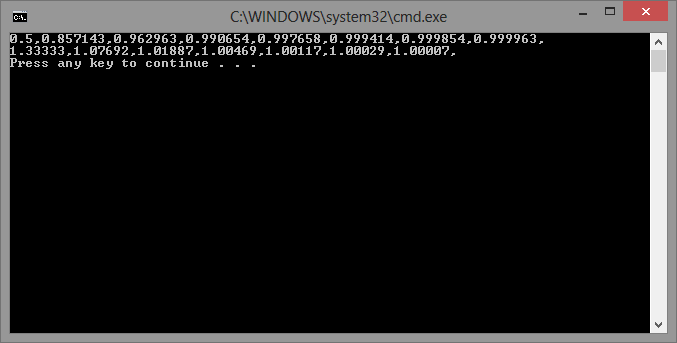
\includegraphics[scale=0.8]{hw4.png} \\
	As we can from the output, the odd sequence is going from $0.5 \rightarrow 1.0$ and the even sequence is 
	going from $1.3 \rightarrow 1.0$ which is quite interesting where $a_1 = \dfrac{1}{2}$
	\begin{proof}
		Consider 
	\end{proof}

		\item Prove that $(a_n)$ converges and find its limit.
	\end{enumerate}
\end{document}
